\newpage
\section{Обработка результатов}
%\label{sec:Chapter5} \index{Chapter5}

\subsection{Оценки качества предсказания}

Допустим, что можно получить качество предсказания классификатора свыше 60\%,
рассматривая электроды по отдельности.
% Предположим, что следующая гипотеза истинна: 
% \begin{equation}
%     \label{eq:hypothesis}
%     \begin{aligned}
%         &\text{рассматривая электроды отдельно друг от друга, можно}\\
%         &\text{получить результат (качество предсказания классификатора),}\\
%         &\text{точность которого свыше 60\%.} 
%     \end{aligned}
% \end{equation}
 
Проанализируем полученные данные.\\
В результате применения линейного метода машинного обучения (логистической регрессии)
на обучающих выборках типа (\ref{eq:eq_2}) получаем следующие результаты, которые
изобразим в виде столбчатой диаграммы:

\begin{figure}[H]
    \centering
    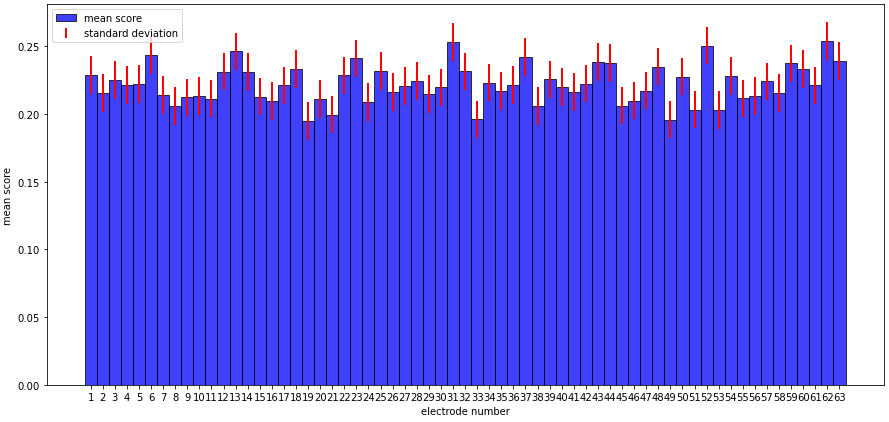
\includegraphics[width=1.05\linewidth]{images/mean_scores.png}
    \caption{Оценки качества предсказания натренированных классификаторов.
    По оси абсцисс --- номера электродов, по оси ординат --- средние по всем участникам
    эксперимента оценки качества предсказания.}
    \label{fig_12}
\end{figure}

Опираясь на изображённую столбчатую диаграмму, можем сформировать представление о том,
как амплитуда биоэлектрической активности, регистрируемой электродом с конкретной зоны
мозга, в отдельности влияет на результат классификации типа решаемой задачи и какие из
них наибольшим образом влияют на результат.

Однако посмотрим на диапазон средних значений оценок качества предсказания
натренированных классификаторов --- варьируется от $\thicksim 0.2$ до $\thicksim 0.25$.
Что интерпретируется следующим образом: доля правильно предсказанных ответов алгоритмом
составляет 20--25\%. Данное утверждение заставляет задуматься о целесообразности
использования в дальнейшем полученных результатов.

Покажем формально, что рассматривать электроды таким образом (то есть по отдельности)
нецелесообразно.

\subsection{P-value}

P-value --- величина, используемая при тестировании статистических гипотез. Фактически
это вероятность ошибки при отклонении нулевой гипотезы (ошибки первого рода) \cite{statistics}.

Пусть $X$ --- множество объектов выборки, $H_0$ --- некоторая нулевая гипотеза, а $T(X)$ --- статистика,
используемая при проверке гипотезы $H_0$. Предполагаем, что если $H_0$ истинна, то распределение
статистики $T(X)$ известно.

Обозначив функцию распределения $F(t)=P(T<t)$, p-value определяется как: $P(t)=2\min(P_{0},P)$.
% % ***********8
% \subsubsection{Формальное определение}

% Пусть есть некоторое значение 
% % здесь подробнее про p-value из wiki
% % ***********

% \begin{figure}[H]
%     \centering
%     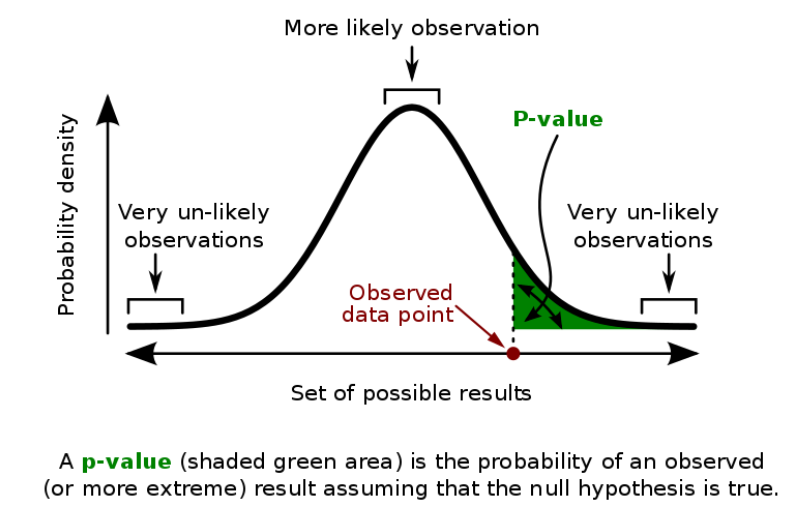
\includegraphics[width=0.8\linewidth]{images/pvalue.png}
%     \caption{Пример вычисления p-value. Вертикальная координата — плотность вероятности
%     каждого результата, вычисленная для нулевой гипотезы. Величина p-value — область под
%     кривой, ограниченной по оси абсцисс наблюдаемой точкой данных.}
%     \label{pvalue}
% \end{figure}


\subsubsection{Применение к логистической регрессии}
\label{sec:chapter_6_2}

Когда мы используем логистическую регрессию, мы используем некоторые независимые
переменные для прогнозирования зависимой переменной (см. главу \ref{sec:chapter_5_2}).
Таким образом, применяя логистическую регрессию, мы получаем коэффициенты для каждой
независимой переменной, которые мы использовали для прогнозирования зависимой переменной.

Рассматривая нашу нулевую гипотезу (cм. главу \ref{sec:hypothesis}) мы предполагаем, что
нет корреляции между признаками и целевыми переменными. В логистической регрессии мы предполагаем, что используемая независимая переменная
(признак) является статистически незначимой (т.е. нет корреляции между признаками
и целевыми переменными) для прогнозирования зависимой переменной или, проще говоря,
её коэффициент корреляции будет равен 0.

Поэтому чем меньше p-value, тем более статистически значимой является рассматриваемая переменная
для нашей модели логистической регрессии.

Допустим, мы получили p-value равное 0.03 или 3\%. Тогда это означает что наши результаты
случайны лишь на 3\% и на столько же не зависят от данного эксперимента. Поэтому, если получим
p-value < 5\%, то придём к выводу, что переменная является значимой и отвергнем нашу
нулевую гипотезу в пользу альтернативной гипотезы.

\subsubsection{Реализация}

Для вычисления p-value воспользовались готовой реализацией statsmodels.
Statsmodels — это python-модуль, который предоставляет классы и функции для оценки
множества различных статистических моделей, а также для проведения статистических тестов
и исследования статистических данных. Для каждой реализации доступен обширный список 
статистики результатов. Результаты проверяются на соответствие существующим статистическим
пакетам, чтобы убедиться в их правильности. Пакет выпущен под лицензией Modified BSD с
открытым исходным кодом \cite{BSD}, \cite{statsmodels}.

\begin{figure}[H]
    \centering
    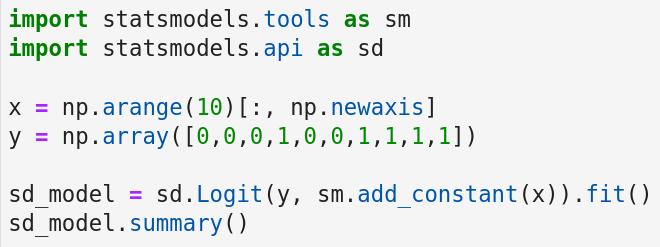
\includegraphics[width=0.7\linewidth]{images/12_2.png}
    \caption{Пример использования готовой реализации для вычисления p-value на языке Python}
    \label{fig_13}
\end{figure}
%
    \let\OriginalVerbatim=\Verbatim
    \makeatletter
    \renewcommand{\Verbatim}[1][1]{%
        %\parskip\z@skip
        \sbox\Wrappedcontinuationbox {\Wrappedcontinuationsymbol}%
        \sbox\Wrappedvisiblespacebox {\FV@SetupFont\Wrappedvisiblespace}%
        \def\FancyVerbFormatLine ##1{\hsize\linewidth
            \vtop{\raggedright\hyphenpenalty\z@\exhyphenpenalty\z@
                \doublehyphendemerits\z@\finalhyphendemerits\z@
                \strut ##1\strut}%
        }%
        % If the linebreak is at a space, the latter will be displayed as visible
        % space at end of first line, and a continuation symbol starts next line.
        % Stretch/shrink are however usually zero for typewriter font.
        \def\FV@Space {%
            \nobreak\hskip\z@ plus\fontdimen3\font minus\fontdimen4\font
            \discretionary{\copy\Wrappedvisiblespacebox}{\Wrappedafterbreak}
            {\kern\fontdimen2\font}%
        }%
        
        % Allow breaks at special characters using \PYG... macros.
        \Wrappedbreaksatspecials
        % Breaks at punctuation characters . , ; ? ! and / need catcode=\active 	
        \OriginalVerbatim[#1,codes*=\Wrappedbreaksatpunct]%
    }
    \makeatother

    % Exact colors from NB
    \definecolor{incolor}{HTML}{303F9F}
    \definecolor{outcolor}{HTML}{D84315}
    \definecolor{cellborder}{HTML}{CFCFCF}
    \definecolor{cellbackground}{HTML}{F7F7F7}
    
    % prompt
    \makeatletter
    \newcommand{\boxspacing}{\kern\kvtcb@left@rule\kern\kvtcb@boxsep}
    \makeatother
    \newcommand{\prompt}[4]{
        {\ttfamily\llap{{\color{#2}[#3]:\hspace{3pt}#4}}\vspace{-\baselineskip}}
    }
    

    
    % Prevent overflowing lines due to hard-to-break entities
    \sloppy 
    % Setup hyperref package
    \hypersetup{
      breaklinks=true,  % so long urls are correctly broken across lines
      colorlinks=true,
      urlcolor=urlcolor,
      linkcolor=linkcolor,
      citecolor=citecolor,
      }
    % Slightly bigger margins than the latex defaults
    
    \geometry{verbose,tmargin=1in,bmargin=1in,lmargin=1in,rmargin=1in}
    
    

\begin{document}
    
    \maketitle
    
    

    
    \begin{tcolorbox}[breakable, size=fbox, boxrule=1pt, pad at break*=1mm,colback=cellbackground, colframe=cellborder]
\prompt{In}{incolor}{1}{\boxspacing}
\begin{Verbatim}[commandchars=\\\{\}]
\PY{k+kn}{import} \PY{n+nn}{numpy} \PY{k}{as} \PY{n+nn}{np}
\PY{k+kn}{from} \PY{n+nn}{scipy}\PY{n+nn}{.}\PY{n+nn}{stats} \PY{k+kn}{import} \PY{n}{norm}
\PY{k+kn}{from} \PY{n+nn}{sklearn}\PY{n+nn}{.}\PY{n+nn}{linear\PYZus{}model} \PY{k+kn}{import} \PY{n}{LogisticRegression}

\PY{k}{def} \PY{n+nf}{logit\PYZus{}pvalue}\PY{p}{(}\PY{n}{model}\PY{p}{,} \PY{n}{x}\PY{p}{)}\PY{p}{:}
    \PY{n}{p1} \PY{o}{=} \PY{n}{model}\PY{o}{.}\PY{n}{predict\PYZus{}proba}\PY{p}{(}\PY{n}{x}\PY{p}{)}
    \PY{n}{n1} \PY{o}{=} \PY{n+nb}{len}\PY{p}{(}\PY{n}{p1}\PY{p}{)}
    \PY{n}{m1} \PY{o}{=} \PY{n+nb}{len}\PY{p}{(}\PY{n}{model}\PY{o}{.}\PY{n}{coef\PYZus{}}\PY{p}{[}\PY{l+m+mi}{0}\PY{p}{]}\PY{p}{)} \PY{o}{+} \PY{l+m+mi}{1}
    \PY{n}{coefs} \PY{o}{=} \PY{n}{np}\PY{o}{.}\PY{n}{concatenate}\PY{p}{(}\PY{p}{[}\PY{n}{model}\PY{o}{.}\PY{n}{intercept\PYZus{}}\PY{p}{,} \PY{n}{model}\PY{o}{.}\PY{n}{coef\PYZus{}}\PY{p}{[}\PY{l+m+mi}{0}\PY{p}{]}\PY{p}{]}\PY{p}{)}
    \PY{n}{x\PYZus{}full} \PY{o}{=} \PY{n}{np}\PY{o}{.}\PY{n}{matrix}\PY{p}{(}\PY{n}{np}\PY{o}{.}\PY{n}{insert}\PY{p}{(}\PY{n}{np}\PY{o}{.}\PY{n}{array}\PY{p}{(}\PY{n}{x}\PY{p}{)}\PY{p}{,} \PY{l+m+mi}{0}\PY{p}{,} \PY{l+m+mi}{1}\PY{p}{,} \PY{n}{axis} \PY{o}{=} \PY{l+m+mi}{1}\PY{p}{)}\PY{p}{)}
    \PY{n}{answ} \PY{o}{=} \PY{n}{np}\PY{o}{.}\PY{n}{zeros}\PY{p}{(}\PY{p}{(}\PY{n}{m1}\PY{p}{,} \PY{n}{m1}\PY{p}{)}\PY{p}{)}
    \PY{k}{for} \PY{n}{i} \PY{o+ow}{in} \PY{n+nb}{range}\PY{p}{(}\PY{n}{n1}\PY{p}{)}\PY{p}{:}
        \PY{n}{answ} \PY{o}{=} \PY{n}{answ} \PYZbs{}
            \PY{o}{+} \PY{n}{np}\PY{o}{.}\PY{n}{dot}\PY{p}{(}\PY{n}{np}\PY{o}{.}\PY{n}{transpose}\PY{p}{(}\PY{n}{x\PYZus{}full}\PY{p}{[}\PY{n}{i}\PY{p}{,} \PY{p}{:}\PY{p}{]}\PY{p}{)}\PY{p}{,} \PY{n}{x\PYZus{}full}\PY{p}{[}\PY{n}{i}\PY{p}{,} \PY{p}{:}\PY{p}{]}\PY{p}{)} \PYZbs{}
            \PY{o}{*} \PY{n}{p1}\PY{p}{[}\PY{n}{i}\PY{p}{,}\PY{l+m+mi}{1}\PY{p}{]} \PY{o}{*} \PY{n}{p1}\PY{p}{[}\PY{n}{i}\PY{p}{,} \PY{l+m+mi}{0}\PY{p}{]}
    \PY{n}{vcov} \PY{o}{=} \PY{n}{np}\PY{o}{.}\PY{n}{linalg}\PY{o}{.}\PY{n}{inv}\PY{p}{(}\PY{n}{np}\PY{o}{.}\PY{n}{matrix}\PY{p}{(}\PY{n}{answ}\PY{p}{)}\PY{p}{)}
    \PY{n}{se} \PY{o}{=} \PY{n}{np}\PY{o}{.}\PY{n}{sqrt}\PY{p}{(}\PY{n}{np}\PY{o}{.}\PY{n}{diag}\PY{p}{(}\PY{n}{vcov}\PY{p}{)}\PY{p}{)}
    \PY{n}{t1} \PY{o}{=}  \PY{n}{coefs}\PY{o}{/}\PY{n}{se}  
    \PY{n}{p1} \PY{o}{=} \PY{p}{(}\PY{l+m+mi}{1} \PY{o}{\PYZhy{}} \PY{n}{norm}\PY{o}{.}\PY{n}{cdf}\PY{p}{(}\PY{n+nb}{abs}\PY{p}{(}\PY{n}{t1}\PY{p}{)}\PY{p}{)}\PY{p}{)} \PY{o}{*} \PY{l+m+mi}{2}
    \PY{k}{return} \PY{n}{p1}

\PY{n}{x} \PY{o}{=} \PY{n}{np}\PY{o}{.}\PY{n}{arange}\PY{p}{(}\PY{l+m+mi}{10}\PY{p}{)}\PY{p}{[}\PY{p}{:}\PY{p}{,} \PY{n}{np}\PY{o}{.}\PY{n}{newaxis}\PY{p}{]}
\PY{n}{y} \PY{o}{=} \PY{n}{np}\PY{o}{.}\PY{n}{array}\PY{p}{(}\PY{p}{[}\PY{l+m+mi}{0}\PY{p}{,}\PY{l+m+mi}{0}\PY{p}{,}\PY{l+m+mi}{0}\PY{p}{,}\PY{l+m+mi}{1}\PY{p}{,}\PY{l+m+mi}{0}\PY{p}{,}\PY{l+m+mi}{0}\PY{p}{,}\PY{l+m+mi}{1}\PY{p}{,}\PY{l+m+mi}{1}\PY{p}{,}\PY{l+m+mi}{1}\PY{p}{,}\PY{l+m+mi}{1}\PY{p}{]}\PY{p}{)}
\PY{n}{model} \PY{o}{=} \PY{n}{LogisticRegression}\PY{p}{(}\PY{n}{C}\PY{o}{=}\PY{l+m+mf}{1e30}\PY{p}{)}\PY{o}{.}\PY{n}{fit}\PY{p}{(}\PY{n}{x}\PY{p}{,} \PY{n}{y}\PY{p}{)}
\PY{n+nb}{print}\PY{p}{(}\PY{n}{logit\PYZus{}pvalue}\PY{p}{(}\PY{n}{model}\PY{p}{,} \PY{n}{x}\PY{p}{)}\PY{p}{)}

\PY{k+kn}{import} \PY{n+nn}{statsmodels}\PY{n+nn}{.}\PY{n+nn}{tools} \PY{k}{as} \PY{n+nn}{sm}
\PY{k+kn}{import} \PY{n+nn}{statsmodels}\PY{n+nn}{.}\PY{n+nn}{api} \PY{k}{as} \PY{n+nn}{sd}
\PY{n}{sd\PYZus{}model} \PY{o}{=} \PY{n}{sd}\PY{o}{.}\PY{n}{Logit}\PY{p}{(}\PY{n}{y}\PY{p}{,} \PY{n}{sm}\PY{o}{.}\PY{n}{add\PYZus{}constant}\PY{p}{(}\PY{n}{x}\PY{p}{)}\PY{p}{)}\PY{o}{.}\PY{n}{fit}\PY{p}{(}\PY{n}{disp}\PY{o}{=}\PY{l+m+mi}{0}\PY{p}{)}
\PY{n+nb}{print}\PY{p}{(}\PY{n}{sd\PYZus{}model}\PY{o}{.}\PY{n}{pvalues}\PY{p}{)}
\PY{n}{sd\PYZus{}model}\PY{o}{.}\PY{n}{summary}\PY{p}{(}\PY{p}{)}
\end{Verbatim}
\end{tcolorbox}

    \begin{Verbatim}[commandchars=\\\{\}]
[0.11413069 0.08780009]
[0.11413093 0.08779979]
    \end{Verbatim}

            \begin{tcolorbox}[breakable, size=fbox, boxrule=.5pt, pad at break*=1mm, opacityfill=0]
\prompt{Out}{outcolor}{1}{\boxspacing}
\begin{Verbatim}[commandchars=\\\{\}]
<class 'statsmodels.iolib.summary.Summary'>
"""
                           Logit Regression Results
==============================================================================
Dep. Variable:                      y   No. Observations:                   10
Model:                          Logit   Df Residuals:                        8
Method:                           MLE   Df Model:                            1
Date:                Sun, 19 Jun 2022   Pseudo R-squ.:                  0.4856
Time:                        22:48:10   Log-Likelihood:                -3.5656
converged:                       True   LL-Null:                       -6.9315
Covariance Type:            nonrobust   LLR p-value:                  0.009472
==============================================================================
                 coef    std err          z      P>|z|      [0.025      0.975]
------------------------------------------------------------------------------
const         -3.9587      2.506     -1.580      0.114      -8.870       0.952
x1             0.8797      0.515      1.707      0.088      -0.130       1.890
==============================================================================
"""
\end{Verbatim}
\end{tcolorbox}
        

    % Add a bibliography block to the postdoc
    
    
    
\end{document}


\begin{figure}[H]
    \centering
    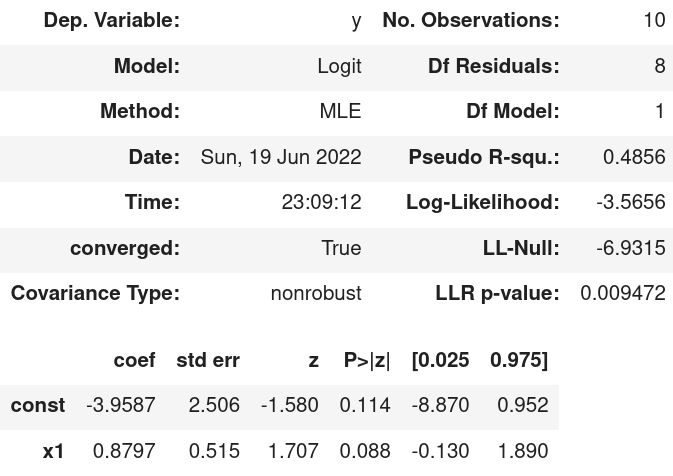
\includegraphics[width=0.7\linewidth]{images/13.png}
    \caption{Вывод работы программы}
    \label{fig_14}
\end{figure}

\subsection{Формулировка гипотезы}

\label{sec:hypothesis}
\begin{flushleft}
    Рассматривая электроды отдельно друг от друга, можно получить результат (качество
    предсказания классификатора), точность которого свыше 60\%.
\end{flushleft} 

% \begin{equation}
%     \label{eq:hypothesis}
%     \begin{aligned}
%         &\text{Рассматривая электроды отдельно друг от друга, можно}\\
%         &\text{получить результат (качество предсказания классификатора),}\\
%         &\text{точность которого свыше 60\%.} 
%     \end{aligned}
% \end{equation}

\subsection{Доказательство}

\subsubsection{Подход №1}
В нашем случае наша гипотеза о том, что с помощью одного электрода можно получить результат,
точность которого больше 60\%
(см. главу\ref{sec:hypothesis}), будет нулевой гипотезой. Тогда альтернативной гипотезой будет 
противоположная ей, о том, что нельзя получить результат с точностью больше 60\%.

Предположим наша нулевая гипотеза истинна. Тогда вычислим p-value для
каждой полученной предсказательной модели. Получим, что максимальное значение по всем
p-value равно 4.8\%, минимальное значение --- 0.7\%, а среднее --- 4.2\% (см. таблицу \ref{fig:table_1}):\\[1 mm]

\begin{table}[H]

    \begin{center}
        \caption{Результаты вычисления p-value}
        \begin{tabular}{ | c | c | c |}
            \hline
            p-value & значение & \% \\ \hline
            max & 0.048 & 4.8\\
            min & 0.007 & 0.7 \\
            mean & 0.042 & 4.2\\
            \hline
        \end{tabular}
        \label{fig:table_1}
    \end{center}
\end{table}

Учитывая, что среднее значение p-value составляет 0.042 или 4.2\%, а p-value каждой модели
не превышает 0.048 или 4.8\% (что меньше 5\%), поэтому мы можем отклонить выдвинутую
гипотезу (нулевую гипотезу) с уровнем значимости 95\% в пользу альтернативной.

\subsubsection{Подход №2}
Используем другой подход. Пусть теперь нулевая гипотеза будет о том, что нельзя получить
точность предсказания классификатора больше 60\%. Вычислим для этого случая p-value.

\begin{table}[H]

    \begin{center}
        \caption{Результаты вычисления p-value}
        \begin{tabular}{ | c | c | c |}
            \hline
            p-value & значение & \% \\ \hline
            max & 0.77 & 77\\
            min & 0.44 & 044 \\
            mean & 0.56 & 56\\
            \hline
        \end{tabular}
        \label{fig:table_2}
    \end{center}
\end{table}

Получив такое p-value нельзя отвергнуть нашу нулевую гипотезу. Данный результат согласуется
с результатом, полученным в предыдущем подходе. Поэтому, рассмотрев несколько подходов, нельзя сказать, что есть хотя бы
один электрод, по которому можно сделать предсказание с точностью свыше 60\%.